\documentclass[../main]{subfiles}

\questiontrue
\solutiontrue

\begin{document}
    \ifquestion
    
	\section{Celestial Chart}

In this exercise, we will discuss a method of cartographic projection for constructing celestial charts, as well as its uses and distortions. For reference, see the figure below, taken from the celestial chart exam of the Vinhedo selection in 2021:

\begin{figure}[htpb]
    \centering
    \includegraphics[scale=0.5]{images/cartx.PNG}
    \caption{Representation of the construction of the projection in question. Source: OBA Selection Committee}
    \label{fig:OBA}
\end{figure}

First, we will find a way to relate the distance of an object to the center of the chart $r$ in relation to the chart radius $R$ and the zenith distance $z$ of the object on the celestial sphere (recall that $h + z = 90^\circ$).

\ut{a} Find the proper relation between $z$ and $r$ as a function of $R$.

\ut{b} Given that the distortion relation $\zeta(z)$ for a zenith distance $z$ is the ratio between an infinitesimal area element on the chart and the corresponding element on the celestial sphere, show that:

$$\zeta(z) = \sec^4{\left(\frac{z}{2}\right)}$$

Kaian, a young astronomer and Marvel fan, was studying the orbits of various satellites around the Earth. For this, he used his faithful "Celestial Chart." As expected, the orbits of the satellites are great circles projected from the center of the Earth onto the celestial sphere.

\ut{c} Kaian wants to know the shape of these orbits on his celestial chart. Therefore, find the shape and the polar and Cartesian equations governing this curve, as a function of the inclination $i$ of the orbit relative to the horizon.

Kaian's disciple, Menegron, was fascinated by geometry and loved calculating areas and angular distances of constellations. To this end, he developed a formula capable of giving the area of a spherical triangle in terms of its internal angles. See Figure \ref{fig:lunulas}:

\clearpage

\begin{figure}[htpb]
    \centering
    \includegraphics{images/luns.PNG}
    \caption{Representation of a generic spherical triangle and its constituent lunes}
    \label{fig:lunulas}
\end{figure}

\ut{d} Argue that the area of a lune\footnote{A lune is one of the two regions between two of these great circles.} formed by two great circles is equal to $2 \alpha R^2$, where $R$ is the radius of the sphere and $\alpha$ is the angle between them.

\ut{e} Using the principle of inclusion and exclusion, show that the area of the spherical triangle $ABC$ is:

$$A_{ABC} = (\alpha + \beta + \gamma - \pi) R^2.$$

On a given night, Menegron noticed that there were 3 satellites on the celestial sphere, with alt-azimuth coordinates (altitude, azimuth): $(90^\circ, 0^\circ)$, $(0^\circ, 97^\circ)$, and $(60^\circ, 187^\circ)$.

\ut{f} Calculate the area of this spherical triangle.

\ut{g} Calculate the projected area of this triangle on the chart.

\ut{h} Show that the ratio between the areas on the chart and on the sphere is:

$$\zeta(\Delta ABC) = 16 - \frac{12 \sqrt{3}}{\pi}$$


\clearpage
\fi
\ifsolution

\section{Celestial Chart}

\ut{a} Consider the system proposed in the figure \ref{fig:nicebitch}.


\begin{figure}[htpb]
    \centering
    

\tikzset{every picture/.style={line width=0.75pt}} %set default line width to 0.75pt        

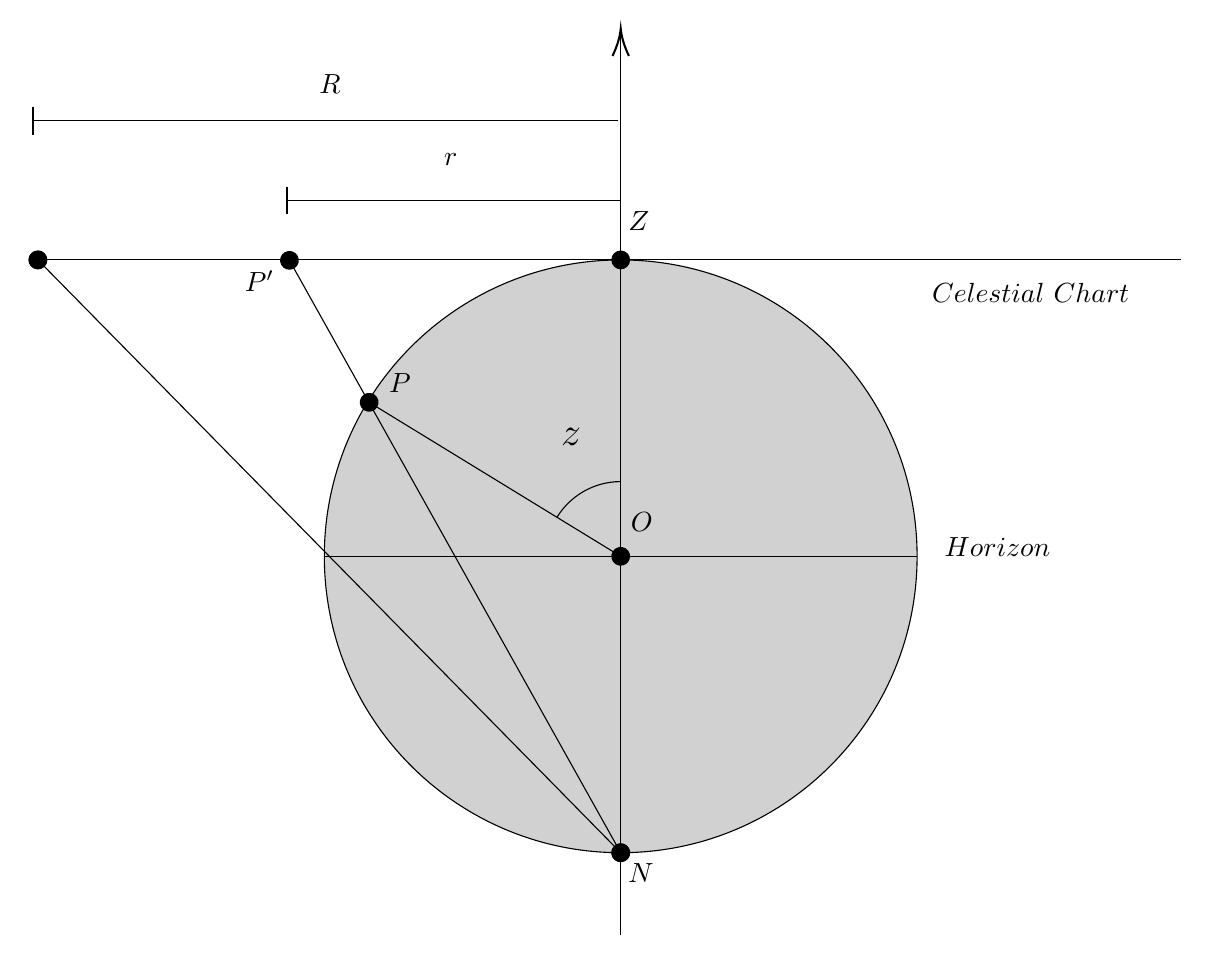
\begin{tikzpicture}[x=0.75pt,y=0.75pt,yscale=-1.2,xscale=1.2]
%uncomment if require: \path (0,643); %set diagram left start at 0, and has height of 643

%Shape: Circle [id:dp9970618795752713] 
\draw  [fill={rgb, 255:red, 155; green, 155; blue, 155 }  ,fill opacity=0.46 ] (206,248) .. controls (206,182.28) and (259.28,129) .. (325,129) .. controls (390.72,129) and (444,182.28) .. (444,248) .. controls (444,313.72) and (390.72,367) .. (325,367) .. controls (259.28,367) and (206,313.72) .. (206,248) -- cycle ;
%Straight Lines [id:da5795924081661066] 
\draw    (91,129) -- (550,129) ;
%Straight Lines [id:da27058793985251683] 
\draw    (325,400.17) -- (325,38.17) ;
\draw [shift={(325,36.17)}, rotate = 90] [color={rgb, 255:red, 0; green, 0; blue, 0 }  ][line width=0.75]    (10.93,-3.29) .. controls (6.95,-1.4) and (3.31,-0.3) .. (0,0) .. controls (3.31,0.3) and (6.95,1.4) .. (10.93,3.29)   ;
%Straight Lines [id:da012450591109866016] 
\draw    (206,248) -- (444,248) ;
%Straight Lines [id:da2889388491395686] 
\draw    (224,186.17) -- (325,248) ;
\draw [shift={(325,248)}, rotate = 31.47] [color={rgb, 255:red, 0; green, 0; blue, 0 }  ][fill={rgb, 255:red, 0; green, 0; blue, 0 }  ][line width=0.75]      (0, 0) circle [x radius= 3.35, y radius= 3.35]   ;
\draw [shift={(224,186.17)}, rotate = 31.47] [color={rgb, 255:red, 0; green, 0; blue, 0 }  ][fill={rgb, 255:red, 0; green, 0; blue, 0 }  ][line width=0.75]      (0, 0) circle [x radius= 3.35, y radius= 3.35]   ;
%Straight Lines [id:da06762538010635644] 
\draw    (192,129.17) -- (325,367) ;
\draw [shift={(325,367)}, rotate = 60.78] [color={rgb, 255:red, 0; green, 0; blue, 0 }  ][fill={rgb, 255:red, 0; green, 0; blue, 0 }  ][line width=0.75]      (0, 0) circle [x radius= 3.35, y radius= 3.35]   ;
\draw [shift={(192,129.17)}, rotate = 60.78] [color={rgb, 255:red, 0; green, 0; blue, 0 }  ][fill={rgb, 255:red, 0; green, 0; blue, 0 }  ][line width=0.75]      (0, 0) circle [x radius= 3.35, y radius= 3.35]   ;
%Shape: Arc [id:dp8935718948531302] 
\draw  [draw opacity=0] (299.42,232.32) .. controls (304.66,223.79) and (314.05,218.08) .. (324.78,218) -- (325,248) -- cycle ; \draw   (299.42,232.32) .. controls (304.66,223.79) and (314.05,218.08) .. (324.78,218) ;  
%Straight Lines [id:da20110494462629247] 
\draw    (91,129) -- (325,367) ;
\draw [shift={(325,367)}, rotate = 45.49] [color={rgb, 255:red, 0; green, 0; blue, 0 }  ][fill={rgb, 255:red, 0; green, 0; blue, 0 }  ][line width=0.75]      (0, 0) circle [x radius= 3.35, y radius= 3.35]   ;
\draw [shift={(91,129)}, rotate = 45.49] [color={rgb, 255:red, 0; green, 0; blue, 0 }  ][fill={rgb, 255:red, 0; green, 0; blue, 0 }  ][line width=0.75]      (0, 0) circle [x radius= 3.35, y radius= 3.35]   ;
%Straight Lines [id:da44548555802041734] 
\draw    (325,105.17) -- (191,105.17) ;
\draw [shift={(191,105.17)}, rotate = 360] [color={rgb, 255:red, 0; green, 0; blue, 0 }  ][line width=0.75]    (0,5.59) -- (0,-5.59)   ;
%Straight Lines [id:da6361213806020154] 
\draw    (324,73.17) -- (89,73.17) ;
\draw [shift={(89,73.17)}, rotate = 360] [color={rgb, 255:red, 0; green, 0; blue, 0 }  ][line width=0.75]    (0,5.59) -- (0,-5.59)   ;
%Straight Lines [id:da4200883890137226] 
\draw    (91,129) -- (325,129) ;
\draw [shift={(325,129)}, rotate = 0] [color={rgb, 255:red, 0; green, 0; blue, 0 }  ][fill={rgb, 255:red, 0; green, 0; blue, 0 }  ][line width=0.75]      (0, 0) circle [x radius= 3.35, y radius= 3.35]   ;
\draw [shift={(91,129)}, rotate = 0] [color={rgb, 255:red, 0; green, 0; blue, 0 }  ][fill={rgb, 255:red, 0; green, 0; blue, 0 }  ][line width=0.75]      (0, 0) circle [x radius= 3.35, y radius= 3.35]   ;

% Text Node
\draw (327,108.57) node [anchor=north west][inner sep=0.75pt]    {$Z$};
% Text Node
\draw (328,229.4) node [anchor=north west][inner sep=0.75pt]    {$O$};
% Text Node
\draw (231,173.4) node [anchor=north west][inner sep=0.75pt]    {$P$};
% Text Node
\draw (300,195.4) node [anchor=north west][inner sep=0.75pt]  [font=\Large]  {$z$};
% Text Node
\draw (173,132.4) node [anchor=north west][inner sep=0.75pt]    {$P'$};
% Text Node
\draw (449,137.4) node [anchor=north west][inner sep=0.75pt]    {$Celestial\ Chart$};
% Text Node
\draw (454,239.4) node [anchor=north west][inner sep=0.75pt]    {$Horizon$};
% Text Node
\draw (327,370.4) node [anchor=north west][inner sep=0.75pt]    {$N$};
% Text Node
\draw (253,85.4) node [anchor=north west][inner sep=0.75pt]    {$r$};
% Text Node
\draw (203,53.4) node [anchor=north west][inner sep=0.75pt]    {$R$};


\end{tikzpicture}
	\caption{Two-dimensional representation of the projection method. $O$ is the origin of the celestial sphere, $N$ is the nadir, $Z$ is the zenith, and $P'$ is the point $P$ projected onto the chart}
    \label{fig:nicebitch}
\end{figure}	

Notice that $\angle POZ = 2 \angle PNO$. From this, we find that:

$$\tan{\left(\frac{z}{2} \right)} = \frac{r}{R}$$

\ut{b} Consider the infinitesimal area element of all points with $z_0 < z < z_0 + dz$. This area will be projected onto the chart such that $r_0 < r < r_0 + dr$.

This area on the celestial sphere is:

$$dA_E = 2\pi \frac{R}{2} \sin{(z)} \frac{R}{2} dz$$

$$dA_E = \frac{\pi R^2}{2} \sin{(z)} dz$$

The projected area on the chart will be:

$$dA_C = 2 \pi r dr$$

So that:

$$\frac{dr}{dz} = R \sec^2{\left( \frac{z}{2}\right)} \frac{1}{2}$$

Thus:

$$dA_C = \pi R^2 \tan{\left(\frac{z}{2} \right)} \sec^2{\left( \frac{z}{2}\right)} dz$$

Finally:

$$\zeta(z) = \frac{dA_C}{dA_E} = \frac{2 \tan{\left(\frac{z}{2} \right)} \sec^2{\left( \frac{z}{2}\right)}}{\sin{(z)}} = \frac{2 \tan{\left(\frac{z}{2} \right)} \sec^2{\left( \frac{z}{2}\right)}}{2 \sin{\left( \frac{z}{2}\right)} \cos{\left( \frac{z}{2}\right)}}$$

$$\zeta(z) = \sec^4{\left(\frac{z}{2}\right)}$$

\ut{c} Given the following orbit with inclination $i$:

\begin{figure}
    \centering
    \includegraphics[scale = 0.9]{images/Orbit.PNG}
    \caption{Spherical triangle of an orbit with inclination $i$}
    \label{fig:inclinedorbit}
\end{figure}

Using spherical trigonometry equations, we have the following relations, using the law of cosines and the law of sines, respectively:

$$\cos{(\omega)} = \cos{(h)}\cos{(\alpha)} + \sin{(\alpha)} \sin{(h)} \cos{(90^\circ)}$$

$$\sin{(h)} = \sin{(i)} \sin{(\omega)}$$

Note that $\sin{(h)} = \cos{(z)}$, $\cos{(h)} = \sin{(z)}$, and $\cos{(90^\circ)} = 0$:

$$\cos{(\omega)} = \sin{(z)} \cos{(\alpha)}$$

$$\cos{(z)} = \sin{(i)} \sin{(\omega)}$$

Squaring both equations and using $\sin^2 x + \cos^2 x = 1$:

$$\cos^2{(\omega)} = \sin^2{(z)} \cos^2{(\alpha)} = 1 - \frac{\cos^2{(z)}}{\sin^2{(i)}}$$

$$\sin^2{(z)} - \sin^2{(z)} \sin^2{(\alpha)} = 1 - \frac{\cos^2{(z)}}{\sin^2{(i)}}$$

$$1 - \cos^2{(z)} - \sin^2{(z)} \sin^2{(\alpha)} = 1 - \frac{\cos^2{(z)}}{\sin^2{(i)}}$$

From this, we find:

$$\sin^2{(\alpha)} = \cos^2{(z)} \left( \frac{1}{\sin^2{(i)}} - 1 \right)$$

Finally:

$$\sin^2{(\alpha)} = \frac{\cot^2{(z)}}{\tan^2{(i)}}$$

However, we have:

$$\tan{(z)} = \frac{2 \tan{\left(\frac{z}{2} \right)}}{1 - \tan^2{\left(\frac{z}{2} \right)}}$$

$$\tan{(z)} = \frac{2 \frac{r}{R}}{1 - \frac{r^2}{R^2}} = \frac{2 R r}{R^2 - r^2}$$

Thus:

$$\sin{(\alpha)} = \frac{R^2 - r^2}{2 R r \tan{(i)}}$$

Converting to Cartesian coordinates:

$$x = r \cos{(\alpha)}$$
$$y = r \sin{(\alpha)}$$

We then notice:

$$y = \frac{R^2 - r^2}{2 R \tan{(i)}}$$

$$r^2 = R^2 - 2 R y \tan{(i)}$$

Since $x^2 = r^2 - y^2$:

$$x^2 = R^2 - 2 R y \tan{(i)} - y^2$$

Completing the equation, we find:

$$x^2 + (y + R \tan{(i)})^2 = (R \sec{(i)})^2$$

Which characterizes a circle.

\ut{d} We can think of a lune as a union of infinitesimal lunes with angle $d\alpha$. Since the areas of these lunes are constant for a constant $d\alpha$, it is expected that the area of the lune is proportional to its opening angle. Hence:

$$A_L = 4 \pi R^2 \frac{\alpha}{2 \pi} = 2 \alpha R^2$$

\ut{e} We can think that the area of the whole sphere is the sum of the areas of the lunes minus 4 times the area of the spherical triangle, since when summing the areas of the lunes we are counting the area of the triangle twice on the front (triangle $ABC$) and twice on the back (the triangle diametrically opposite $ABC$). This implies:

$$4 \pi R^2 = 2(2 \alpha R^2 + 2 \beta R^2 + 2 \gamma R^2) - 4 A_{ABC}$$

Therefore:

$$A_{ABC} = (\alpha + \beta + \gamma - \pi) R^2$$

\ut{f} It is easy to see that the angles of this triangle are $90^\circ$, $90^\circ$, and $30^\circ$:

\begin{figure}[htpb]
    \centering
    \includegraphics[scale = 0.8]{images/FB.PNG}
    \caption{Representation of the spherical triangle proposed in the problem statement}
    \label{fig:crazyshiit}
\end{figure}

Thus:

$$A_{ABC} = \left( \frac{\pi}{2} + \frac{\pi}{2} + \frac{\pi}{6} - \pi \right) \frac{R^2}{4}$$

$$A_{ABC} = \frac{\pi R^2}{24}$$

\ut{g} For this item, we need to project each point onto the chart and find the area between them, knowing that the sides will be circles (or straight lines, which correspond to circles of infinite radius). For this, observe the desired projection:


	\begin{figure}[htpb]
	    \centering
	    

\tikzset{every picture/.style={line width=0.75pt}} %set default line width to 0.75pt        

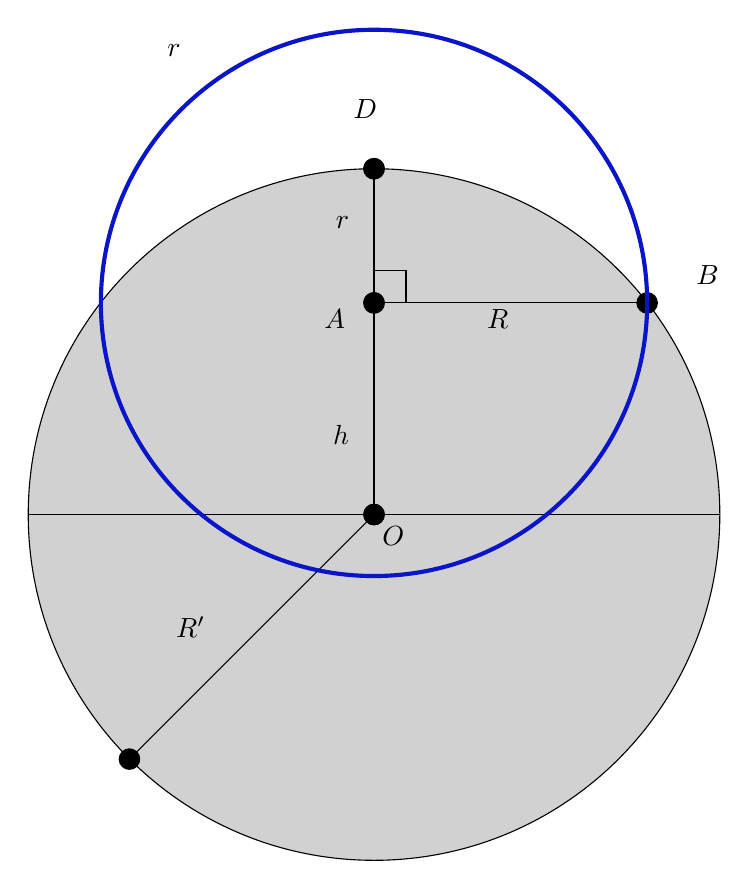
\begin{tikzpicture}[x=0.75pt,y=0.75pt,yscale=-1.4,xscale=1.4]
%uncomment if require: \path (0,643); %set diagram left start at 0, and has height of 643

%Shape: Circle [id:dp9970618795752713] 
\draw  [fill={rgb, 255:red, 155; green, 155; blue, 155 }  ,fill opacity=0.46 ] (206,248) .. controls (206,182.28) and (259.28,129) .. (325,129) .. controls (390.72,129) and (444,182.28) .. (444,248) .. controls (444,313.72) and (390.72,367) .. (325,367) .. controls (259.28,367) and (206,313.72) .. (206,248) -- cycle ;
%Straight Lines [id:da012450591109866016] 
\draw    (206,248) -- (444,248) ;
%Straight Lines [id:da2889388491395686] 
\draw    (325,129) -- (325,248) ;
\draw [shift={(325,248)}, rotate = 90] [color={rgb, 255:red, 0; green, 0; blue, 0 }  ][fill={rgb, 255:red, 0; green, 0; blue, 0 }  ][line width=0.75]      (0, 0) circle [x radius= 3.35, y radius= 3.35]   ;
\draw [shift={(325,129)}, rotate = 90] [color={rgb, 255:red, 0; green, 0; blue, 0 }  ][fill={rgb, 255:red, 0; green, 0; blue, 0 }  ][line width=0.75]      (0, 0) circle [x radius= 3.35, y radius= 3.35]   ;
%Straight Lines [id:da06762538010635644] 
\draw    (325,129) -- (325,175.17) ;
\draw [shift={(325,175.17)}, rotate = 90] [color={rgb, 255:red, 0; green, 0; blue, 0 }  ][fill={rgb, 255:red, 0; green, 0; blue, 0 }  ][line width=0.75]      (0, 0) circle [x radius= 3.35, y radius= 3.35]   ;
\draw [shift={(325,129)}, rotate = 90] [color={rgb, 255:red, 0; green, 0; blue, 0 }  ][fill={rgb, 255:red, 0; green, 0; blue, 0 }  ][line width=0.75]      (0, 0) circle [x radius= 3.35, y radius= 3.35]   ;
%Straight Lines [id:da20110494462629247] 
\draw    (325,175.17) -- (419,175.17) ;
\draw [shift={(419,175.17)}, rotate = 0] [color={rgb, 255:red, 0; green, 0; blue, 0 }  ][fill={rgb, 255:red, 0; green, 0; blue, 0 }  ][line width=0.75]      (0, 0) circle [x radius= 3.35, y radius= 3.35]   ;
\draw [shift={(325,175.17)}, rotate = 0] [color={rgb, 255:red, 0; green, 0; blue, 0 }  ][fill={rgb, 255:red, 0; green, 0; blue, 0 }  ][line width=0.75]      (0, 0) circle [x radius= 3.35, y radius= 3.35]   ;
%Straight Lines [id:da4200883890137226] 
\draw    (325,248) -- (240.83,332.17) ;
\draw [shift={(240.83,332.17)}, rotate = 135] [color={rgb, 255:red, 0; green, 0; blue, 0 }  ][fill={rgb, 255:red, 0; green, 0; blue, 0 }  ][line width=0.75]      (0, 0) circle [x radius= 3.35, y radius= 3.35]   ;
\draw [shift={(325,248)}, rotate = 135] [color={rgb, 255:red, 0; green, 0; blue, 0 }  ][fill={rgb, 255:red, 0; green, 0; blue, 0 }  ][line width=0.75]      (0, 0) circle [x radius= 3.35, y radius= 3.35]   ;
%Shape: Circle [id:dp047168026616374314] 
\draw  [color={rgb, 255:red, 10; green, 20; blue, 200 }  ,draw opacity=1 ][line width=1.5]  (231,175.17) .. controls (231,123.26) and (273.09,81.17) .. (325,81.17) .. controls (376.91,81.17) and (419,123.26) .. (419,175.17) .. controls (419,227.09) and (376.91,269.17) .. (325,269.17) .. controls (273.09,269.17) and (231,227.09) .. (231,175.17) -- cycle ;
%Shape: Square [id:dp2693176967038797] 
\draw   (325,164.17) -- (336,164.17) -- (336,175.17) -- (325,175.17) -- cycle ;

% Text Node
\draw (327,251.4) node [anchor=north west][inner sep=0.75pt]    {$O$};
% Text Node
\draw (311,144.4) node [anchor=north west][inner sep=0.75pt]    {$r$};
% Text Node
\draw (307,176.4) node [anchor=north west][inner sep=0.75pt]    {$A$};
% Text Node
\draw (253,85.4) node [anchor=north west][inner sep=0.75pt]    {$r$};
% Text Node
\draw (363,176.4) node [anchor=north west][inner sep=0.75pt]    {$R$};
% Text Node
\draw (310,216.4) node [anchor=north west][inner sep=0.75pt]    {$h$};
% Text Node
\draw (256,282.4) node [anchor=north west][inner sep=0.75pt]    {$R'$};
% Text Node
\draw (435,161.4) node [anchor=north west][inner sep=0.75pt]    {$B$};
% Text Node
\draw (317,104.4) node [anchor=north west][inner sep=0.75pt]    {$D$};


\end{tikzpicture}
	
    \caption{Projection of the orbital circle onto the celestial chart}
    \label{fig:cartx}
\end{figure}

Denote point $A$ as the vertex of the triangle at the zenith, point $B$ as the point on the horizon, and point $D$ as the point with altitude $60^\circ$. As explained earlier, the side $DB$ of the spherical triangle is projected onto a circle passing through $D$ and $B$.

The area of this element $ADB$ is given by the area of the circular sector $ODB$ minus the area of the triangle $OAB$, where $O$ is the center of the larger circle. Notice that $h = R \tan{(i)}$ from the equation of the larger circle, so the angle $AÔB$ is:

$$\tan{(AÔB)} = \cot{(i)}$$

Which implies: $AÔB = 90^\circ - i$. The area of the sector is:

$$A_S = \frac{1}{2} \left( \frac{\pi}{2} - i \right) R^2 \sec^2{(i)}$$

The area of the triangle is:

$$A_T = \frac{1}{2} R^2 \tan{(i)}$$

So the lune area is:

$$A_l = \frac{1}{2} \left( \frac{\pi}{2} - i \right) R^2 \sec^2{(i)} - \frac{1}{2} R^2 \tan{(i)} = \frac{R^2}{2} \left( \frac{\pi}{2} \sec^2{(i)} - i \sec^2{(i)} - \tan{(i)} \right)$$

Since $i = 60^\circ$:

$$A_l = \frac{R^2}{2} \left( \frac{4 \pi}{3} - \sqrt{3} \right)$$

\ut{h} Hence:

	$$\zeta{(\Delta ABC)}=\frac{12\left(\frac{4\pi}{3} - \sqrt{3} \right) }{\pi}$$
	
	$$\zeta{(\Delta ABC)}=16-\frac{12\sqrt{3}}{\pi} \approx 9.38$$
	
	\clearpage
    
    
    \fi
\end{document}
